\documentclass{ctexart}
\usepackage[spanish]{babel}
\usepackage{graphicx}
\graphicspath{{imgs/}}
\title{Minería de textos} % Sets article title
\author{Pelayo Martínez} % Sets authors name
\date{\today} % Sets date for publication as date compiled

% The preamble ends with the command \begin{document}
\begin{document} % All begin commands must be paired with an end command somewhere

	\maketitle % creates title using information in preamble (title, author, date)
    
	%New section is created
	\section{Tema 1}
    La \textbf{minería de textos} es el proceso de analizar colecciones de textos para descubrir información y patrones que no aparecen de forma explícita en los textos.
    Engloba: 
	\begin{itemize}
	\item   \textbf{Extracción de información}: consiste en extraer automáticamente información estructurada a partir de textos.
	\item   \textbf{Recuperación de información}: consiste en buscar documentos, buscar información dentro de los documentos y en buscar metadatos que describan los documentos. Incluye la búsqueda en todo tipo de repositorios y bases de datos, tanto aisladas como conectadas en red
	\item   \textbf{Categorización}: consiste en asignar a un documento una o más categorías en función de su contenido. Las categorías con las que se hace la clasificación están definidas previamente.
	\item   \textbf{Agrupamiento de documentos}: es una forma de organización de documentos en grupos en la que ni la naturaleza de los grupos, ni en ocasiones su número están definidos de antemano
	\end{itemize}
		
	\begin{flushleft}
	La minería de textos se aplica a colecciones de documentos con información textual no estructurada y escrita en lenguaje natural. Esta información normalmente conforma documentos que pueden agruparse en colecciones o corpus.  Se utilizan principalmente técnicas de procesamiento del lenguaje natural y de aprendizaje automático.
	\end{flushleft}
	\begin{flushleft}
	\textbf{Procesamiento del lenguaje natural (PLN)}: rama de la informática cuyo objetivo es el desarrollo de sistemas que permitan a los ordenadores comunicarse con personas utilizando el lenguaje humano. Se utiliza para adquirir conocimientos a partir de cantidades masivas de datos textuales (generar resumenes, sistemas de dialogo, etc). 
	\end{flushleft}
	Es difícil porque:

	\begin{itemize}
	\item Alta ambigüedad a todos los niveles (léxico, sintáctico, semántico y de discursos): El entendimiento del lenguaje permite evitar estas ambigüedades.
	\item Ciertos aspectos intervienen en la interpretación (saber si se niega la información, si es especulativa, expresiones que hacen referencia a una misma cosa, etc)
	\end{itemize}

	\subsection{Evaluación de tareas de PLN}
	Para evaluar datos de los modelos es necesario comparar modelos y sistemas (sobre sorpus o colecciones comunes o bien usando las mismas medidas)
	Un \textbf{corpus} es una compilación de textos en formato electrónico. Son fundamentales para el desarrollo de aplicaciones basadas en PLN, ya que permiten evaluar sistemas y entrenan sistemas de aprendizaje automático.
	Son muestras amplias y naturales del lenguaje y a su vez fuente de datos estadísticos sobre palabras, relaciones y construcciones.
	Hay 2 tipos de corpus:
	\begin{itemize}
		\item \textbf{Sin anotar}: Texto puro
		\item \textbf{Anotados}: Marcados con información lingüística (se les conoce como \textit{Gold standard} y se usan de referencia)
	\end{itemize}
	También cabe destacar la distinción respecto al contenido:
	\begin{itemize}
		\item \textbf{Paralelos}: Mismos textos en distintos idiomas
		\item \textbf{Comparables}: Contienen un número equilibrado (en cuanto al tema y al tipo) de textos en distintos idiomas
	\end{itemize}
	\textbf{Campañas de evaluación}: Proponen retos a los participantes, proporcionando datos y un marco de evaluación común y bien definido.
	\begin{itemize}
		\item \textbf{TREC}: Evaluan metodologías de recuperación de textos a gran escala.
		\item \textbf{CLEF}: Promueven la investigación y desarrollo de sistemas de acceso a información.
		\item \textbf{Semeval}: Evaluan sistemas de análisis semántico.
		\item \textbf{Iberval/Iberlef}: Organizan campañas de evaluación en castellano y otras lenguas ibéricas.
	\end{itemize}
	\subsection{Medidas de evaluación más habituales}
	\begin{flushleft}
		\textbf{Precisión}: Fracción de predicciones del modelo propuesto acertadas (coinciden con los datos de referencia)\par
		\begin{displaymath}
		p = \frac{tp}{tp+fp} 
		\end{displaymath}
		*donde tp: true positive y fp: false positive\par
		\textbf{Cobertura o exhaustividad (recall)}: Fracción de los datos de referencia que han sido propuestas por el modelo evaluado\par
		\begin{displaymath}
		r = \frac{tp}{tp+fn} 
		\end{displaymath}
		*donde fn: false negative\par
		\textbf{Medida-F}: Media armónica de precisión y cobertura\par
		\begin{displaymath}
		Medida-F = \frac{2 \cdot p \cdot r}{p+r} 
		\end{displaymath}\par
		\textbf{Medida-F}β: Forma general de la media armónica que permite dar más importancia a la precisión o a la cobertura en función del parámetro β. \par
		\begin{displaymath}
		Medida-F_{\beta}  = (1+\beta^2) \frac{p \cdot r}{\beta^2 \cdot p + r} 
		\end{displaymath}
		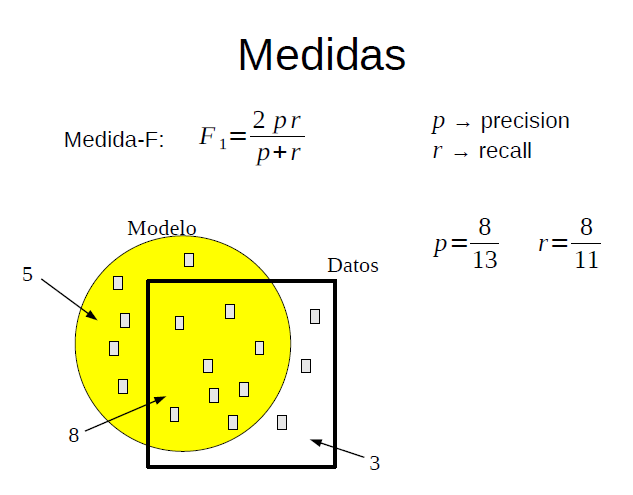
\includegraphics[scale=0.75]{medidas}
	\end{flushleft}
	\subsection{Baseline}
	\begin{flushleft}
		La baseline es la medida de los resultados de un modelo básico que resuelve la tarea. Es importante tener una referencia para saber qué niveles de las medidas se consideran aceptables.
		Ejemplo:
		\begin{itemize}
			\item Tarea: asignar el significado correcto a una palabra ambigua en el contexto de un documento.
			\item Baseline: asignar el significado más frecuente de la palabra.	Se espera que cualquier otro modelo propuesto supere la baseline
		\end{itemize}
	\end{flushleft}
	\subsection{Análisis de errores}
	\begin{flushleft}
		Permite encontrar errores en los programas, en los datos de entrenamiento y es fundamental para desarrollar nuevos modelos de conocimiento o algoritmos de resolución de problemas.
		Las \textbf{matrices de confusión} se utilizan para analizar errores en los clasificadores. Una matriz de confusión para una tarea de clasificación de N clases es una matriz de NxN
		donde la celda(x,y) contiene el número de veces que un elemento con la clasificación correcta x fue clasificado por el modelo como y.
		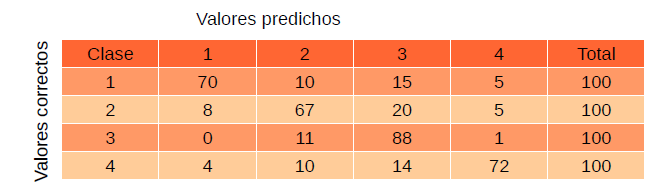
\includegraphics[scale=0.75]{errores}
	\end{flushleft}
	\subsection{Introducción al procesamiento del lenguaje natural}
	\begin{flushleft}
	Las fases del procesamiento del lenguaje son:
	\begin{enumerate}
		\item Procesamiento de textos
		\begin{enumerate}
			\item Expresiones regulares
			\item Normalización
			\item Distancia de edición
		\end{enumerate}
		\item POS tagging
		\item Stemming
		\item Chunking
		\item Desambiguación del sentido de las palabras
	\end{enumerate}
	\end{flushleft}
	\subsection{Expresiones regulares}
	\begin{flushleft}
		Las expresiones regulares son un lenguaje formal para especificar patrones de texto.
	\end{flushleft}
	\subsection{Normalización}
	\begin{flushleft}
		Existen 2 tipos de normalización:
		\begin{itemize}
			\item Normalización de textos: Proceso de transformación del texto para obtener una forma canónica. El objetivo es uniformizar la forma del texto para facilitar posteriores procesos.
			Técnicas comunes:
			\begin{enumerate}
				\item Normalización de la forma de las palabras
				\item Tokenización de oraciones
				\item Tokenización de palabras
			\end{enumerate}
			\item Normalización de palabras: Proceso de unificación de palabras que se refieren de distinta	forma a la misma entidad (forman una clase común).
			Técnicas comunes:
			\begin{enumerate}
				\item Eliminar acentos
				\item Quitar espacios repetidos
				\item Reducir todas las palabras a minúsculas
			\end{enumerate}
		\end{itemize}
	\end{flushleft}
	\subsection{Distancia de edición}
	\begin{flushleft}
		La distancia de edición es la distancia mínima entre 2 cadenas para convertir una en la otra. Se usa para la correción de errores ortográficos, para extraer información, para traducir automáticamente, etc. \par 
		Posee distintas operaciones:
		\begin{itemize}
			\item Inserción
			\item Borrado
			\item Sustitución
		\end{itemize}
		Se necesita explorar todas las combinaciones de	operación para seleccionar la de menor coste. Ejemplo: \par
		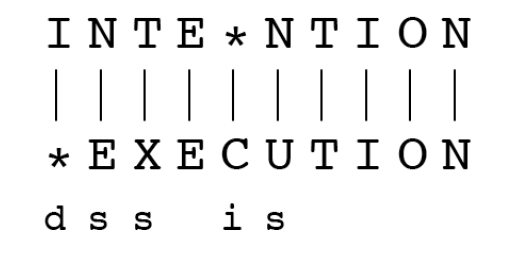
\includegraphics[scale=0.5]{dedicion} \par
		Si cada operación tiene coste 1: la distancia es 5. \par
		Si la sustitución tiene coste 2, la distancia es 8
	\end{flushleft}
	\subsection{Palabras vacías}
	\begin{flushleft}
		Son palabras vacías aquellas sin significado propio: artículos, preposiciones, etc. Suelen ser las más frecuentes en un idioma. En muchos PLN se eliminan para centrar el análisis en palabras con contenido semántico.
	\end{flushleft}
	\subsection{Segmentación}
	\begin{flushleft}
		Se usa para romper cadenas de caracteres (grafemas) en secuencias de palabras.  Las claves para segmentar el texto son la puntuación (puntos, signos de interrogación y signos de exclamación). A veces se aborda junto
		a la tokenización de palabras dado que los puntos pueden delimitar oraciones o marcar abreviaturas (se suelen usar diccionarios de abreviaturas para ayudar a saber de qué tipo de punto se trata).
	\end{flushleft}
	\subsection{Análisis morfológico}
	\begin{flushleft}
		La \textbf{morfológía} es el campo de la lingüística que estudia la estructura de las palabras. \par
		Un \textbf{morfema} es la unidad lingüística más pequeña que tiene significado semántico. \par
		El \textbf{análisis morfológico} es la tarea de segmentar una palabra en sus morfemas. \par
		Los morfemas pueden ser \textbf{raices} y \textbf{afijos} (prefijos y sufijos). La raíz es el morfema principal que da significado a la palabra. El afijo añade significado adicional (número, género, tiempo verbal, etc). \par
		perros → perr + o + s 
	\end{flushleft}
	\subsection{Stemming}
	\begin{flushleft}
		El proceso de \textbf{stemming} se refiere al proceso de eliminar la parte final de las palabras, que en muchas ocasiones es una aproximación a la lematización.
		La \textbf{lematización} es el proceso de identificar el lema o forma canónica de una palabra (leíamos -> leer)
	\end{flushleft}
	\subsection{POS tagging}
	\begin{flushleft}
		El etiquetado gramatical o \textbf{Part-Of-Speech (POS) Tagging} es el proceso de etiquetar las palabras de una oración con su categoría léxica, en base a:
		\begin{itemize}
			\item Su definción
			\item El contexto en la oración (las etiquetas y palabras que la rodean)
		\end{itemize}
		Este proceso es muy util para identificar entidades, desambiguar el sentido de las palabras, analisis sintáctico, etc. Se evalua mediante:
		\begin{itemize}
			\item La exactitud (accuracy): número de etiquetas acertadas sobre el número total de palabras etiquetadas
			\item Precisión, cobertura y medida-F para cada tipo de	etiqueta del conjunto de etiquetas considerado
		\end{itemize}
		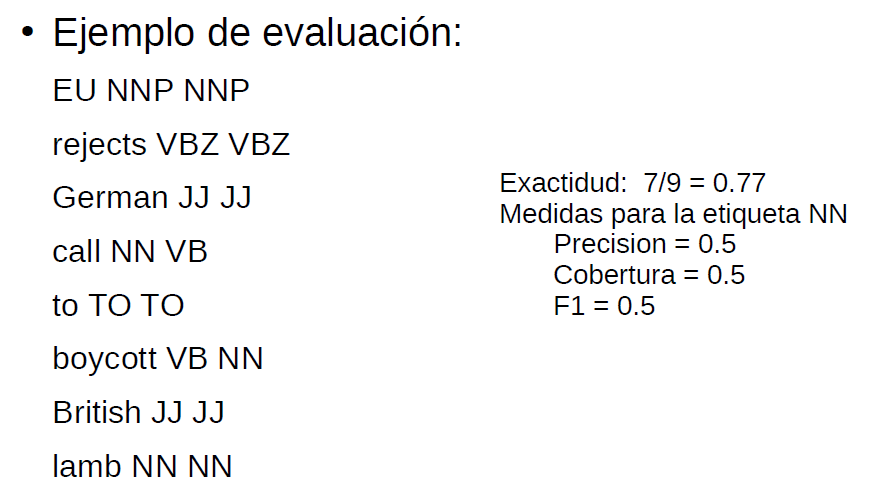
\includegraphics[scale=0.35]{evalpos} \par
	\end{flushleft}
	\subsection{Chunking}
	\begin{flushleft}
		Se trata del proceso de partir y etiquetar secuencias multipalabra (cada secuencia es un chunk). Uno de los más usados es el de las frases nominales (NP chunking)
	\end{flushleft}
	\subsection{Análisis sintáctico}
	\begin{flushleft}
		Tiene como objetivo identificar la estructura sintáctica de una oración (dependiendo del tipo de gramática considerada). Se usa en sistemas de extracción de información, sistemas de búsqueda de respuestas, etc. \par 
		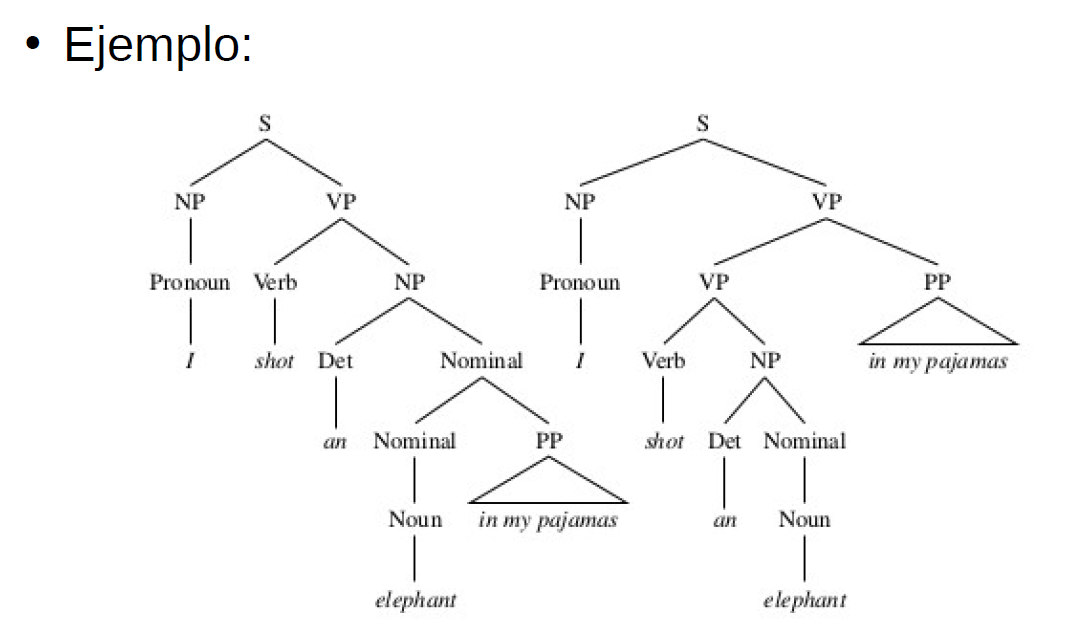
\includegraphics[scale=0.35]{sintac} \par
	\end{flushleft}
	\subsection{Análisis de constituyentes}
	\begin{flushleft}
		Una frase bien formada se puede descomponer en constituyentes de acuerdo a unas reglas gramaticales. Un analizador sintáctico de constituyentes es un programa que obtiene la estructura asociada a una frase respecto a una gramática. \par 
	\end{flushleft}
	\subsection{Desambiguación del sentido de las palabras}
	\begin{flushleft}
		Muchas palabras tienen más de un significado o sentido dependiendo del contexto en que se usan:
		\begin{itemize}
			\item Los pescadores encontraron un gran banco de sardinas
			\item Tuve que ir al banco a sacar dinero
			\item Nos sentamos en el banco hasta que llegó
		\end{itemize}
		La desambiguación del sentido de las palabras consiste en seleccionar el sentido (interpretación o significado) correcto de una ocurrencia de una palabra en un documento (o conversación) de entre todos los posibles de la palabra. \par 
		Aplicaciones:
		\begin{itemize}
			\item Traducción automática: es necesaria las palabras que tienen diferentes traducciones para diferentes sentidos
			\item Recuperación de información: es necesario desambiguar las	consultas: depresión puede hacer referencia una enfermedad, a una situación económica, etc.
			\item Extracción de información: para la interpretación correcta de los textos. Drug puede hacer referencia a un medicamento o a una sustancia ilegal.
		\end{itemize}
	\end{flushleft}
\end{document} % This is the end of the document